\documentclass[12pt,compress,aspectratio=169]{beamer}
\input{../../mybeamer}
\usepackage{pgfplots}

\usetikzlibrary{decorations.pathmorphing,patterns}

\title{Class 13: Harmonic Motion, Part 2}
\subtitle{AP Physics C--Mechanics}
\input{../../me}
\input{../../mycommands}


\begin{document}

\begin{frame}
  \maketitle
\end{frame}


\section{Damped Oscillation}

\begin{frame}{It's Never Perfect}
  In reality, there are friction, or drag, or other damping forces present in
  the spring-mass system, represented schematically by the shock absorber:
  \begin{center}
    \begin{tikzpicture}
      \draw[gray,mass] (3,.5) rectangle (4,1.5);
      \draw[thick,draw=gray,decorate,
        decoration={aspect=.4,segment length=5,amplitude=8,coil}] (0,1)--(3,1);
      \fill[gray,pattern=north east lines] (-.2,2)--(-.2,.3)--(6.7,.3)--(6.7,2)
      --(6.5,2)--(6.5,.5)--(0,.5)--(0,2)--cycle;
      \draw[gray,thick] (0,2)--(0,.5)--(6.5,.5)--(6.5,2);
      \draw[axes] (7.25,1)--(8,1) node[right]{$x$};
      \fill[blue!20!white] (5,.8) rectangle (6,1.2);
      \draw[very thick] (4,1)--(5,1);
      \draw[very thick] (5,.8)--(5,1.2);
      \draw[very thick] (4.9,1.2)--(6,1.2)--(6,.8)--(4.9,.8);
      \draw[very thick] (6,1)--(6.5,1);

      \draw[vectors,pink] (3.5,1)--(3.5,0) node[right]{$\vec F_g$};
      \draw[vectors,pink] (3.5,1)--(3.5,2) node[right]{$\vec F_n$};
      \draw[vectors,pink] (3.5,1)--(2.5,1) node[above]{$\vec F_s$};
      \draw[vectors,red] (3.5,1)--(4.5,1) node[above]{$\vec F_D$};
      \fill[red] (3.5,1) circle (.075);
    \end{tikzpicture}
  \end{center}
  The combined friction, drag, and damping forces are grouped into a single
  damping force ``$\vec F_D$''.
  
  %\uncover<3->{
  %  \vspace{-.1in}The damping force is typically related to velocity, in the
  %  opposite direction:
  %
  %  \eq{-.135in}{
  %    F_D=-bv^n
  %  }
  %
  %  \vspace{-.12in}where $b$ is a positive constant called the \textbf{damping
  %    factor}.
    %The simplest case is to use $n=1$ to represent combined viscous
    %effects. %(Kinetic friction, $n=0$; aerodynamic drag, $n=2$)
  %}
\end{frame}



\begin{frame}{Damped Oscillators}
  In general, the damping force is a function of velocity, and acts in the
  opposite direction to the motion of the mass:
  
  \eq{-.22in}{
    F_D=-bv^n
  }

  \vspace{-.15in}The positive constant $b$ is called the \textbf{damping
    factor}.
  \begin{itemize}
  \item For kinetic friction, $n=0$
  \item For aerodynamic drag, $n=2$, and
  \item For viscous damping, $n\approx 1$
  \end{itemize}
  Usually there is a combination of these forces, so we use $n=1$ to
  approximate the \emph{average}\footnote{Whether this is
  \emph{accurate} will depend on the specific problem that needs to be solved.}.
  %Applying the 2nd law of motion, the differential equation is more complicated:
  %
  %\eq{-.2in}{
  %  -kx-bv=ma
  %}
\end{frame}




\begin{frame}{Damped Oscillator}
  The 2nd-order ODE is obtained by applying second law of motion, this time
  with the additional term from the damping force:

  \eq{-.1in}{
    \sum F=F_s+{\color{red}F_D}=ma\quad\rightarrow\quad
    -kx{\color{red}-b\diff xt}=m\diff[2]xt
  }

  Arranging into standard form:
  
  \eq{-.1in}{
    \diff[2]xt+\frac bm\diff xt+\frac kmx=0
  }

  The solution to this ODE is still relatively straightforward (but not as
  easy).
\end{frame}



\begin{frame}{Damped Oscillator}
  The solution to this ODE\footnote{This is still a standard problem in
    calculus.} has both an {\color{magenta}exponential decay term} and a
  {\color{cyan}sinusoidal term}:

  \eq{-.1in}{
    x(t)=\underbracket[1pt]{A_0{\color{magenta}e^{-\frac b{2m}t}}}_\text{amplitude}
    {\color{cyan}\cos(\omega t+\phi)}
  }

  where $A_0$ is the initial amplitude of the damped oscillator,
  and the ``natural frequency'' for the damped oscillator is given by:

  \eq{-.1in}{
    \omega=\sqrt{\omega_0^2-\left(\frac b{2m}\right)^2}
  }
  
  Note that $\omega<\omega_0$ (natural frequency decreases) because of the
  damping factor $b$.
  \vspace{.3in}
\end{frame}



\begin{frame}{Critical Damping}
  \textbf{Critical damping} occurs when the natural frequency $\omega$ is zero,
  i.e.:
  
  \eq{-.1in}{
    \sqrt{\omega_0^2-\left(\frac{b_c}{2m}\right)^2}=0
  }

  which corresponds to the \textbf{critical damping constant} $b_c$:

  \eq{-.1in}{
    b_c=2m\omega_0%=2\sqrt{km}
  }
  \begin{itemize}
  \item A critically damped system returns to its equilibrium position in the
    shortest time with \emph{no} oscillation
  \item When $b>b_c$, the system is \textbf{over-damped}
  \item Critical or near-critical damping is desired in many engineering
    designs (e.g.\ shock absorbers on car suspensions)
  \end{itemize}
\end{frame}



\begin{frame}{Comparing Damped System}
  \centering
  \pic{.5}{oscda8}
  
  The motion of the damped oscillator is not strictly periodic.
\end{frame}



%\begin{frame}{Energy in a Damped System}
%  The non-conservative damping force dissipates energy from the oscillator at
%  a rate of:
%
%  \eq{-.1in}{
%    P=\diff Et=\vec F_D\cdot\vec v=-bv^2
%  }
%
%  As velocity relate to energy by: $(v_{av})^2=E/m$, power dissipation is a
%  first-order linear ODE:
%
%  \eq{-.1in}{
%    \diff Et=-\frac bmE
%  }
%
%  The solution to the ODE shows the total amount of energy decreases
%  exponentially with time:
%
%  \eq{-.1in}{
%    E(t)=E_0e^{-\frac bmt} %=E_0e^{-\frac{t}{\tau}}
%    }
%\end{frame}



\section{Driven Oscillation}

\begin{frame}{Forced Harmonic Motion}
  To keep a damped system going, energy must be added into the system. Assuming
  that the system is subjected to an external applied force ($F_a$) that is
  harmonic with time, with a driving frequency $\omega_\text{ext}$:

  \eq{-.2in}{
    F_a=F\cos(\omega_\text{ext}t)
  }
  
  \vspace{-.2in}
  \begin{center}
    \begin{tikzpicture}
      \draw[gray,mass] (3,.5) rectangle (4,1.5);
      \draw[thick,gray,decorate,
        decoration={aspect=.4,segment length=6,amplitude=8,coil}] (0,1)--(3,1);
      \fill[gray,pattern=north east lines] (-.5,2)--(-.5,.3)--(6.7,.3)--(6.7,2)
      --(6.5,2)--(6.5,.5)--(0,.5)--(0,2)--cycle;
      \draw[gray,thick] (0,2)--(0,.5)--(6.5,.5)--(6.5,2);
      \draw[fill=blue!10] (4.9,.8) rectangle (5.5,1.2);
      \draw[very thick,gray] (4,1)--(4.9,1);
      \draw[very thick,gray] (4.9,.8)--(4.9,1.2);
      \draw[very thick,gray] (4.8,1.2)--(5.5,1.2)--(5.5,.8)--(4.8,.8);
      \draw[very thick,gray] (5.5,1)--(6.5,1);
      \draw[vectors,pink] (3.5,1)--(3.5,0) node[right]{$\vec F_g$};
      \draw[vectors,pink] (3.5,1)--(3.5,2) node[right]{$\vec F_n$};
      \draw[vectors,pink] (3.5,1)--(2.5,1) node[above]{$\vec F_s$};
      \draw[vectors,red] (3.5,.95)--(2,.95) node[below]{$\vec F_a$};
      \draw[vectors,pink] (3.5,1)--(4.5,1) node[below]{$\vec F_D$};
      \fill[red] (3.5,1) circle (.075);
    \end{tikzpicture}
  \end{center}
  In general, the driving frequency $\omega_\text{ext}$ is unrelated to the
  undamped natural frequency $\omega_0$ or damped natural frequency $\omega$.
\end{frame}



\begin{frame}{Forced Harmonic Motion}
  Again, the second-order ordinary differential equation is obtained by
  applying the second law of motion:
  
  \eq{-.1in}{
    \sum F=-kx-bv+F\cos(\omega_\text{ext}t)=ma
  }

  Rearranging the terms gives a similar ODE to the damped oscillator, but with
  the {\color{magenta}additional applied external force term} on the right-hand
  side:

  \eq{-.1in}{
    m\diff[2]xt+b\diff xt+kx={\color{magenta}F\cos(\omega_\text{ext}t)}
  }
\end{frame}



\begin{frame}{Forced Harmonic Motion}
  This is a much more difficult problem in calculus, but nevertheless still a
  standard problem
  
  \eq{-.1in}{
    m\diff[2]xt + b\diff xt+kx=F\cos(\omega_\text{ext} t)
  }
  
  The solution to this ODE has two components:
  \begin{itemize}
  \item A \textbf{transient solution} that is identical to that of the damped
    oscillator
    \begin{itemize}
    \item Obtained by setting $F_a=0$
    \item Depends on the initial condition
    \item Solution becomes negligible over time because of exponential-decay
    \end{itemize}
  \item A \textbf{steady-state solution} which does not depend on the initial
    condition
  \end{itemize}
\end{frame}



\begin{frame}{Forced Harmonic Motion}
  Solving for the steady-state solution will be left as a difficult calculus
  exercise\footnote{This is usually taught in a 2nd-year university level ODE
  course}, but it can be shown that the solution is a harmonic motion at the
  driving frequency $\omega_\text{ext}$ of the external force:

  \eq{-.1in}{
    \boxed{x(t)=A\cos(\omega_\text{ext}t-\phi)}
  }
  
  where the amplitude of the oscillation $A$ and phase shift $\phi$ are given
  by:

  \eq{-.05in}{
    A=\frac F{\sqrt{m^2(\omega_0^2-\omega_\text{ext}^2)^2+b^2\omega_\text{ext}^2}}
    \quad\quad
    \tan\phi=\frac{b\omega_\text{ext}}{m(\omega_0^2-\omega_\text{ext}^2)}
  }
  \vspace{.5in}
\end{frame}



\begin{frame}{Amplitude Response to External Driving Force}
  The amplitude of the driven oscillation is given by:
  
  \eq{-.1in}{
    A=\frac F{\sqrt{m^2(\omega_0^2-\omega_\text{ext}^2)^2+b^2\omega_\text{ext}^2}}
  }
  
  Maximum $A$ occurs when the denominator is minimized, i.e.\ when the
  derivative with respect to external frequency $\omega_\text{ext}$ is 0:

  \eq{-.25in}{
    \diff{}{\omega_\text{ext}}\left[m^2(\omega_0^2-\omega_\text{ext}^2)^2+b^2\omega_\text{ext}^2\right]=0
    \;\;\longrightarrow\;\;
    \omega_\text{ext}=\sqrt{\omega_0^2-\frac{b^2}{2m^2}}\approx\omega
  }

  The driving frequency $\omega_\text{ext}$ when amplitude is maximum occurs at a
  frequency that is very close to (albeit slightly different from) the natural
  frequency of the damped system.
\end{frame}



\begin{frame}{Resonance}
  \begin{columns}
    \column{.5\textwidth}
    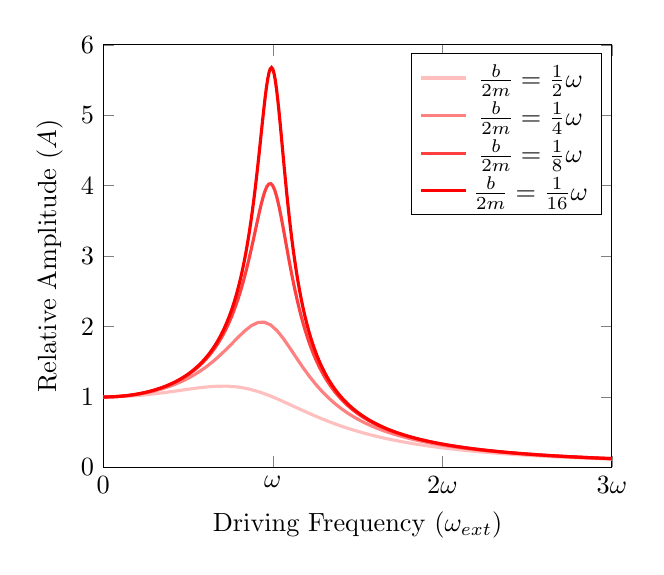
\begin{tikzpicture}[scale=.95]
      \begin{axis}[
          width=3.3in,
          xmin=0,xmax=3, xlabel=Driving Frequency ($\omega_\text{ext}$),
          xtick={0,1,2,3}, xticklabels={0,$\omega$,$2\omega$,$3\omega$},
          ymin=0,ymax=6, ylabel=Relative Amplitude ($A$),
          ytick={0,1,2,3,4,5,6}
        ]
        \addplot[
          color=red!25,
          samples=50,
          domain=0:3,
          very thick]{1/sqrt((1-x^2)^2+x^2)};
        \addlegendentry{$\frac b{2m}=\frac12\omega$}
        \addplot[
          color=red!50,
          samples=80,
          domain=0:3,
          very thick]{1/sqrt((1-x^2)^2+x^2/4)};
        \addlegendentry{$\frac b{2m}=\frac14\omega$}
        \addplot[
          color=red!75,
          samples=250,
          domain=0:3,
          very thick]{1/sqrt((1-x^2)^2+x^2/16)};
        \addlegendentry{$\frac b{2m}=\frac18\omega$}
        \addplot[
          color=red,
          samples=400,
          domain=0:3,
          very thick]{1/sqrt((1-x^2)^2+x^2/32)};
        \addlegendentry{$\frac b{2m}=\frac1{16}\omega$}
      \end{axis}
    \end{tikzpicture}

    \column{.5\textwidth}
    Plotting amplitude $A$ as a function of driving frequency
    $\omega_\text{ext}$ shows that:
    \begin{itemize}
    \item For a lightly damped system (i.e.\ small $b$), resonance response is
      highest when $\omega_\text{ext}\approx\omega\approx\omega_0$
    \item The smaller the damping constant $b$, the higher and narrower the
      peak is
    \end{itemize}
  \end{columns}
\end{frame}



\begin{frame}{Resonance}
  \eq{0in}{
    \boxed{\tan\phi=\frac{b\omega_a}{m(\omega_0^2-\omega_\text{ext}^2)}}
  }

  When $\omega_\text{ext}=\omega_0$ is substituted into the phase shift
  expression, the right-hand side becomes undefined. From this, we obtain a
  phase shift of $\phi=\pi/2$. Taking derivative of $x(t)$ for velocity $v(t)$,
  and substituting $\phi=\pi/2$:
  
  \eq{-.1in}{
    v(t)=\dot x
    =-A\omega_\text{ext}\sin(\omega_\text{ext}t-\frac{\pi}2)
    =A\omega_\text{ext}\cos(\omega_\text{ext}t)
  }
\end{frame}



\begin{frame}{Resonance}
  At resonance, the object is always moving in the same direction as the
  driving force:

  \vspace{-.3in}{\large
    \begin{align*}
      v(t)&=A\omega_\text{ext}\cos(\omega_\text{ext} t)\\
      F_a(t)&=F\cos(\omega_\text{ext} t)
    \end{align*}
  }

  This also makes sense from a work-energy perspective, because now the
  external force is doing positive work to the system.
\end{frame}



\begin{frame}{Resonance}
  \textbf{Resonance} is caused by in-phase excitation near the natural
  frequency. This means that:
  \begin{itemize}
  \item The frequency of the driving force is \emph{approximately} equal to the
    natural frequency of the damped oscillator:

    \eq{-.1in}{
      \omega_\text{ext}=\sqrt{\omega_0^2-\frac{b^2}{2m^2}}
      \quad\text{where}\quad\omega_0=\sqrt{\frac km}
    }

    For a lightly damped system, $\omega_\text{ext}\approx\omega\approx\omega_0$
  \item The driving force follows the motion of the oscillator.
  \end{itemize}
\end{frame}
\end{document}
